\documentclass[a4paper, 12pt, twoside]{article}
\usepackage[utf8]{inputenc}		% LaTeX, comprend les accents !
\usepackage[T1]{fontenc}		
\usepackage[francais]{babel}
\usepackage{lmodern}
\usepackage{ae,aecompl}
\usepackage[top=2.5cm, bottom=2cm, 
			left=2cm, right=2cm,
			headheight=15pt]{geometry}
\usepackage{graphicx}
\usepackage{eso-pic}	% Nécessaire pour mettre des images en arrière plan
\usepackage{array} 
\usepackage{hyperref}
\usepackage{lastpage}
\usepackage[acronym,toc]{glossaries}
\begin{titlepage}


	\begin{center}
	
		
		\begin{figure}[H]
		\begin{center}
			\includegraphics[scale=0.6]{logouvsq.png}
	
		\end{center}
		
	\end{figure}
		
		\large{\emph{{{ \it \bf {Rapport de projet Numérique }}}}}\\
		\vspace{0.1cm}
		\normalsize
		\begin{center}
	
			Domaine : \textbf{Calcul Haute Performance, Simulation} \\
			Filière : \textbf {Calcul Haute Performance, Simulation}\\
	
		\end{center}
		
		
		\vspace{0.09cm}
		\Huge{Thème}\\
		\noindent\rule{\textwidth}{0.1mm}
		\Large{{\textbf{Utilisation et analyse critique des rapports MAQAO pour optimiser des mini-apps}}}
		\noindent\rule{\textwidth}{0.1mm}
	\end{center}
	\begin{center}
		\normalsize %\hspace{-2cm}
		\vspace{1.5cm}

		\begin{tabular}{llll}

			\vspace{0.09cm}
			\textbf{Présenté par :} \hspace{9cm} \textsl{\textbf{Proposé et encadré par :}}\\
			\vspace{0.1cm}
			$M^{r}$ \textsl{Anis MEHIDI}
			\hspace{9cm}\textsl{$M^{r}$ Cedric VALENCI}\\ 
		    $M^{r}$ \textsl{Arezki Takfarines HAMIDANI}
		    \hspace{6.5cm}\textsl{$M^{r}$  Emmanuel OSERET}\\
		    $M^{me}$ \textsl{Katia MOALI }\\
		    $M^{r}$ \textsl{Madjid BOUZOURENE}\\
		    $M^{me}$ \textsl{Sylia BENBACHIR}\\
		    

	
\usepackage{tcolorbox,listings}
\usepackage{fullpage}
\usepackage{color}
 
\definecolor{darkWhite}{rgb}{0.94,0.94,0.94}
 
\lstset{
    backgroundcolor=\color{darkWhite},
    breakatwhitespace=false,
    breaklines=true,
    captionpos=b,
    commentstyle=\color{red},
    deletekeywords={...},
    escapeinside={\%*}{*)},
    extendedchars=true,
    keepspaces=true,
    keywordstyle=\color{blue},
    language=C,
    morekeywords={*,...},
    showspaces=false,
    showstringspaces=false,
    showtabs=false,
    stepnumber=1,
    stringstyle=\color{gray},
    tabsize=4,
    title=\lstname,
}
 
\lstdefinestyle{frameStyle}{
    basicstyle=\footnotesize,
    numbers=left,
    numbersep=20pt,
    numberstyle=\tiny\color{black}
}
 
\tcbuselibrary{listings,skins,breakable}
 
\newtcblisting{customFrame}{
    arc=0mm,
    top=0mm,
    bottom=0mm,
    left=3mm,
    right=0mm,
    width=\textwidth,
    listing only,
    listing options={style=frameStyle},
    breakable
}

\author{}
\title{Le titre du rapport de stage}
\entreprise{MAQAO}
\fonction{}
\datedebut{26 mars 2018}
\datefin{date de fin du stage}

\date{placer ici la date de la soutenance}
\jurya{}{}{}

%\juryd{M. Prénom Nom}{poste de votre maître de stage}{Maître de stage}
%Ajouter le juryd si votre maître de stage viens accompagné d'un collègue.
\makeglossaries % Avant que les termes et acronymes soient définis
\loadglsentries{glossaire}

\begin{document}
\pagedegarde


%placer vos remerciements ici


%La table des matières
\tableofcontents
\newpage
\listoffigures
%--------------------------liste des figures

\newpage

\section{Introduction}

\section{Maqao sur un cas simple : Nbody3D}


Afin de réaliser notre rapport PPN, il était nécessaire de comprendre le fonctionnement des différents flags d'optimisation des compilateurs de MAQAO et d'apprendre à l'utiliser. Pour cela, nous avons cherché à optimiser un benchmark déjà vu en cours : \textbf{Nbody3D}. L'idée était de faire le travail d'optimisation un maximum de fois depuis la version de base afin d'identifier les informations récurrentes et
exploitable qui nous étaient produites.


\subsection{Code source}

\subsubsection{Makefile}
La version de base du Makefile qui nous était donnée, il est compliqué et exécuté sans aucune optimisation.
	
\begin{customFrame}
all: nbody.g
nbody.g: nbody.c
	gcc -g -mavx2 -fopt-info-all=nbody.gcc.optrpt $< -o $@ -lm -fopenmp
clean:
	rm -Rf *~ nbody.g  *.optrpt

\end{customFrame}


\subsubsection{Nbody.c}

\begin{customFrame}
//
#include <omp.h>
#include <math.h>
#include <stdio.h>
#include <stdlib.h>

//
typedef float              f32;
typedef double             f64;
typedef unsigned long long u64;

//
typedef struct particle_s {

  f32 x, y, z;
  f32 vx, vy, vz;
  
} particle_t;

//
void init(particle_t *p, u64 n)
{
  for (u64 i = 0; i < n; i++)
    {
      //
      u64 r1 = (u64)rand();
      u64 r2 = (u64)rand();
      f32 sign = (r1 > r2) ? 1 : -1;
      
      //
      p[i].x = sign * (f32)rand() / (f32)RAND_MAX;
      p[i].y = (f32)rand() / (f32)RAND_MAX;
      p[i].z = sign * (f32)rand() / (f32)RAND_MAX;

      //
      p[i].vx = (f32)rand() / (f32)RAND_MAX;
      p[i].vy = sign * (f32)rand() / (f32)RAND_MAX;
      p[i].vz = (f32)rand() / (f32)RAND_MAX;
    }
}

//
void move_particles(particle_t *p, const f32 dt, u64 n)
{
  //
  const f32 softening = 1e-20;

  //
  for (u64 i = 0; i < n; i++)
    {
      //
      f32 fx = 0.0;
      f32 fy = 0.0;
      f32 fz = 0.0;

      //23 floating-point operations
      for (u64 j = 0; j < n; j++)
	{
	  //Newton's law
	  const f32 dx = p[j].x - p[i].x; //1
	  const f32 dy = p[j].y - p[i].y; //2
	  const f32 dz = p[j].z - p[i].z; //3
	  const f32 d_2 = (dx * dx) + (dy * dy) + (dz * dz) + softening; //9
	  const f32 d_3_over_2 = pow(d_2, 3.0 / 2.0); //11

	  //Net force
	  fx += dx / d_3_over_2; //13
	  fy += dy / d_3_over_2; //15
	  fz += dz / d_3_over_2; //17
	}

      //
      p[i].vx += dt * fx; //19
      p[i].vy += dt * fy; //21
      p[i].vz += dt * fz; //23
    }

  //3 floating-point operations
  for (u64 i = 0; i < n; i++)
    {
      p[i].x += dt * p[i].vx;
      p[i].y += dt * p[i].vy;
      p[i].z += dt * p[i].vz;
    }
}

//
int main(int argc, char **argv)
{
  //
  const u64 n = (argc > 1) ? atoll(argv[1]) : 16384;
  const u64 steps= 10;
  const f32 dt = 0.01;

  //
  f64 rate = 0.0, drate = 0.0;

  //Steps to skip for warm up
  const u64 warmup = 3;
  
  //
  particle_t *p = malloc(sizeof(particle_t) * n);

  //
  init(p, n);

  const u64 s = sizeof(particle_t) * n;
  
  printf("\n\033[1mTotal memory size:\033[0m %llu B, %llu KiB, %llu MiB\n\n", s, s >> 10, s >> 20);
  
  //
  printf("\033[1m%5s %10s %10s %8s\033[0m\n", "Step", "Time, s", "Interact/s", "GFLOP/s"); fflush(stdout);
  
  //
  for (u64 i = 0; i < steps; i++)
    {
      //Measure
      const f64 start = omp_get_wtime();

      move_particles(p, dt, n);

      const f64 end = omp_get_wtime();

      //Number of interactions/iterations
      const f32 h1 = (f32)(n) * (f32)(n - 1);

      //GFLOPS
      const f32 h2 = (23.0 * h1 + 3.0 * (f32)n) * 1e-9;
      
      if (i >= warmup)
	{
	  rate += h2 / (end - start);
	  drate += (h2 * h2) / ((end - start) * (end - start));
	}

      //
      printf("%5llu %10.3e %10.3e %8.1f %s\n",
	     i,
	     (end - start),
	     h1 / (end - start),
	     h2 / (end - start),
	     (i < warmup) ? "*" : "");
      
      fflush(stdout);
    }

  //
  rate /= (f64)(steps - warmup);
  drate = sqrt(drate / (f64)(steps - warmup) - (rate * rate));

  printf("-----------------------------------------------------\n");
  printf("\033[1m%s %4s \033[42m%10.1lf +- %.1lf GFLOP/s\033[0m\n",
	 "Average performance:", "", rate, drate);
  printf("-----------------------------------------------------\n");
  
  //
  free(p);

  //
  return 0;
}
\end{customFrame}




\newpage
\subsection{Déroulement du processur d'optimisation}
\subsubsection{Étape Initiale}
Dans la première étape, nous allons effectuer une analyse binaire en utilisant les flags permettant à MAQAO de faire son analyse. Après ça, on va utiliser les informations obtenues afin d'améliorer les performances de notre programme en suivant les différentes indications du rapport MAQAO.

\subsubsection*{La page Index}
    
    On commence notre analyse par la page d'accueil du rapport. Comme on peut l'observer, on retrouve des informations qui sont utiles afin d'optimiser notre programme.
    \begin{enumerate}
        \item[1.]Global Metrics
        
         On suit cette lecture afin de savoir ce qu'il faut faire: 
    \begin{enumerate}
        \item[\textbullet]Pour les informations en vert: quand la valeur est bonne.
        \item[\textbullet] Pour les informations en orange claire: quand la valeur est bonne mais qu'elle peut s'améliorer.
        \item[\textbullet]Pour les informations en orange: lorsque la valeur est moyenne et montre un problème de performance potentiel.
        \item[\textbullet]Pour les informations en rouge: lorsque la valeur est mauvaise et montre probablement un problème de performances, on doit impérativement les rajouter\\ afin d'avoir un rapport efficace.
    \end{enumerate}
    
    
    \begin{figure}[h]
    \centering
    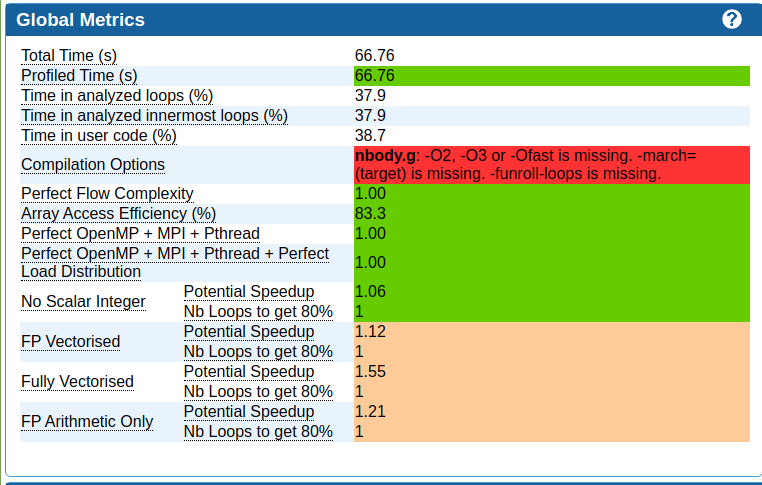
\includegraphics[width=\textwidth]{Figures/cap1.png}
    \caption{Global Metrics.}
    
    \end{figure}
    \newpage
    En analysant le Global Metrics de notre programme, on constate ces points:
    \begin{enumerate}
        \item[\textbullet]Que ce programme est compilé sans flags d'optimisation et on doit impérativement les utiliser pour avoir un programme optimisé.
        \item[\textbullet]Que notre Array Access Efficiency est efficace qu'a 75\%, alors qu'on devrait avoir un 100\%.
        \item[\textbullet]Que les Speedup peuvent-être meilleure si le programme est vectorisé à la compilation et ils doivent être à 1.
        \item[\textbullet]
    \end{enumerate}
    
A cette étape, nous allons prendre en compte la suggestion des flags [O2, O3, Ofast], -march=target et -funroll-loops pour le prochain programme à produire.
    
        \item[2.]Experiment Summary
         \begin{figure}[h]
    \centering
    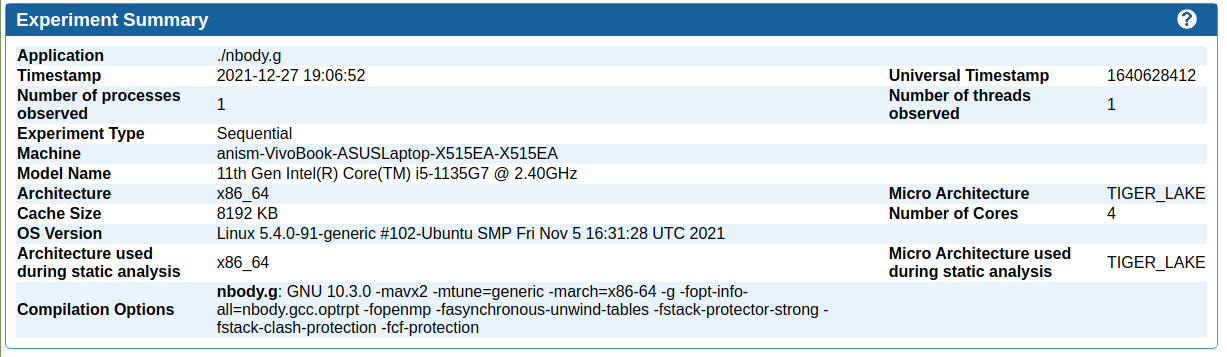
\includegraphics[width=\textwidth]{Figures/cap2.png}
    \caption{Experiment Summary.}
    
    \end{figure}
    
    
    Dans les options de compilation, on voit que le flag -march existe avec x86-64, car il utilise la version de base de -march et pour que notre programme soit optimisé, on doit le modifier à -march=target
    \end{enumerate}
   

   \subsubsection*{La page Loops}
   A cette étape, nous savons que notre code est peut être optimisable et que les Speedups sont intéressants et que nous pouvons les améliorer, c'est dans cette étape qu'on va découvrir.
            \begin{figure}[h]
    \centering
    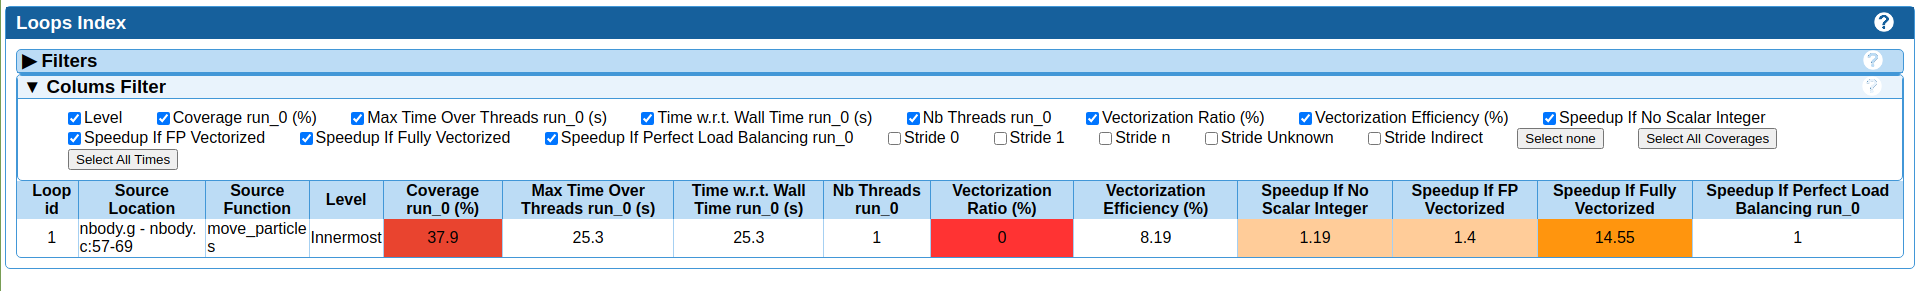
\includegraphics[width=\textwidth,height=4cm]{Figures/cap3.png}
    \caption{Loops Index.}
    
    \end{figure}
    \newpage
    
    
   Comme on peut le voir, on a un tableau récapitulatif des boucles que nous devrons optimiser, ici dans notre cas on a une seule boucle qui nous pose problème, avec un Coverage de 37.9\% et une vectorisation de 0\% et des speedup que nous devrons améliorer et qui doivent être à 1.
   
   
   Pour savoir ce qu'il faut modifier exactement, MAQAO nous donne des étapes à suivre dans le rapport CQA.
   
   \subsubsection*{Rapport CQA}
   Le rapport CQA se présente comme le montre la figure suivante:
         \begin{figure}[h]
    \centering
    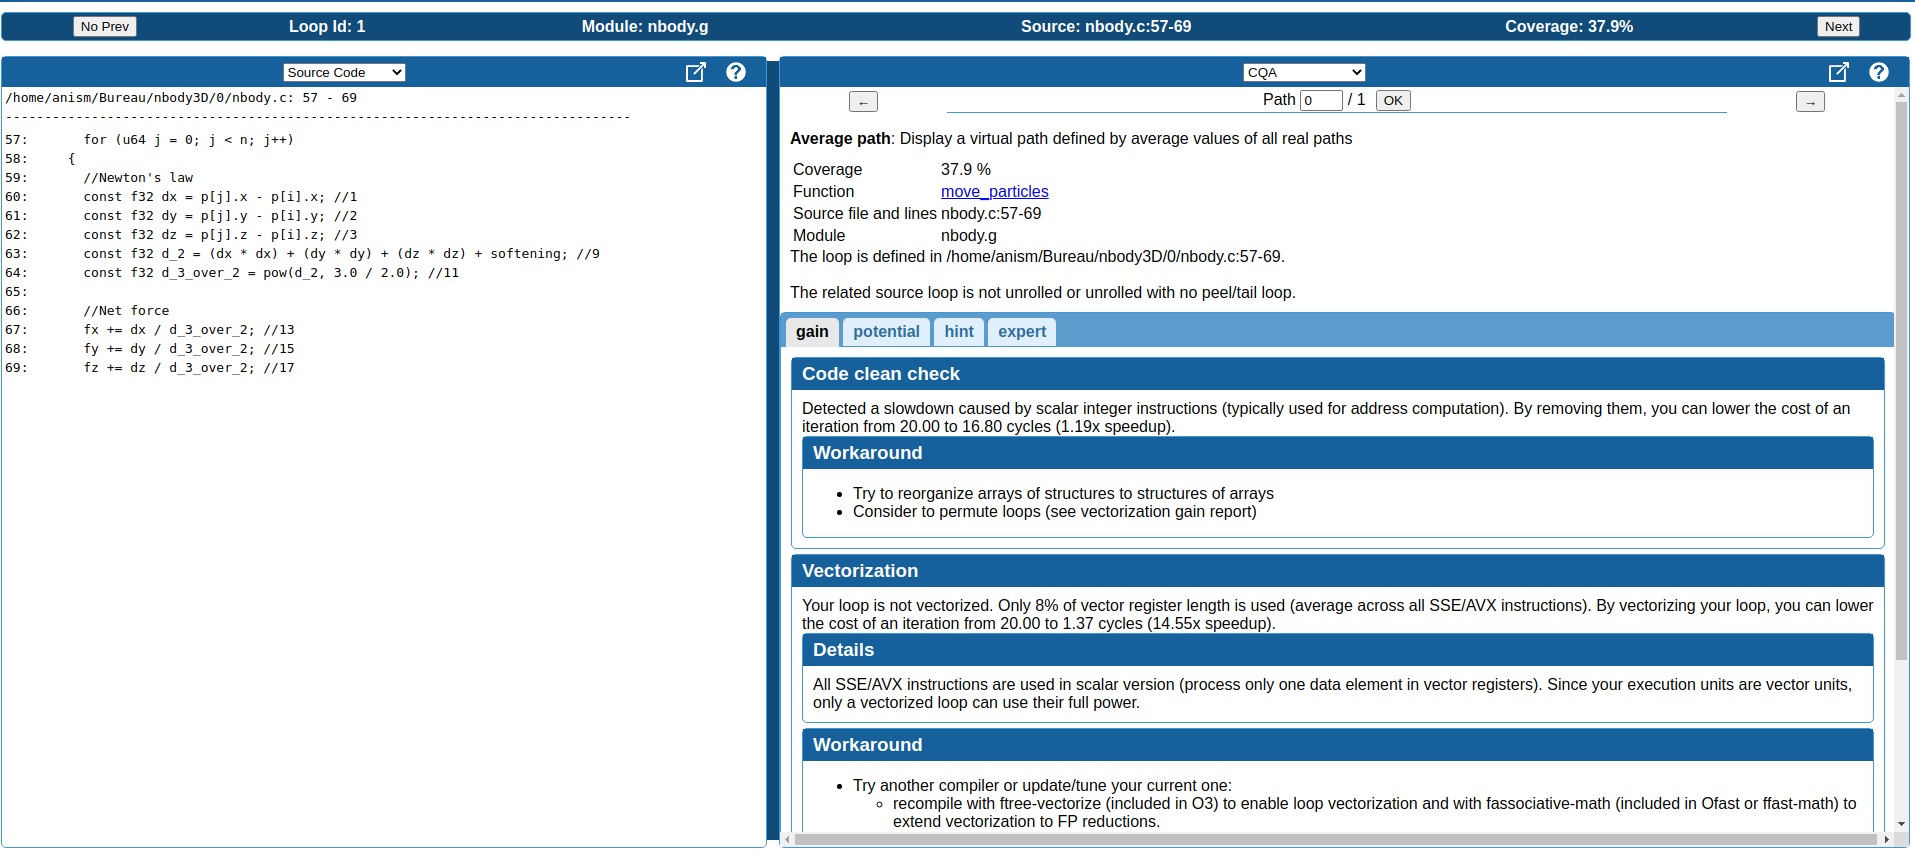
\includegraphics[width=\textwidth]{Figures/cap4.png}
    \caption{Rapport CQA de la boucle N°1.}
    
    \end{figure}
    On peut voir le code source de la boucle sur la gauche et les améliorations à effectué dessus sur la droite. Nous allons réaliser chacune des modifications
demandée lorsque cela est possible afin de pouvoir constater dans une analyse ultérieur si notre programme est optimisé.
\begin{enumerate}
    \item[\textbullet]\textbf{Gain : Code clean check}
    
    Dans cette section, ça nous montre qu'il y'a un ralentissement causé par des instructions d'entier scalaire (généralement utilisées pour le calcul d'adresse). En les supprimant, nous pouvons réduire le coût d'une itération.
       \begin{figure}[h]
    \centering
    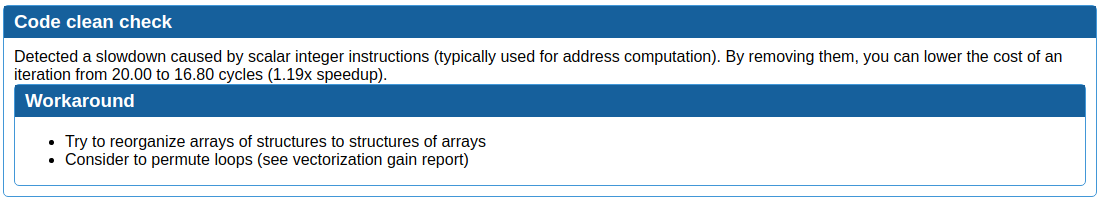
\includegraphics[width=\textwidth]{Figures/cap5.png}
    \caption{Gain : Code clean check.}
    
    \end{figure}
    
    \newpage
    \item[\textbullet]\textbf{Gain : Vectorization}
    
    Dans cette section, on nous montre que notre boucle n'est pas du tout vectorisé, il nous montre les instructions à suivre afin d'avoir une vectorisation meilleure, en prenant en compte des flags d'optimisation \textbf{ftree-vectorize} et \textbf{fassociative-math} et aussi changer la structure du code qui est en AOS (Array of Structures) en SOA( Structures of Array).
    
        \begin{figure}[h]
    \centering
    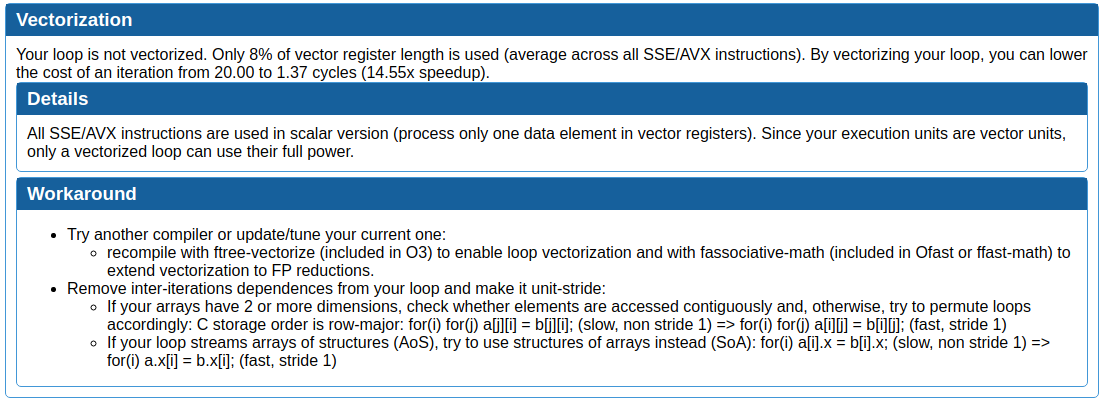
\includegraphics[width=\textwidth]{Figures/cap6.png}
    \caption{Gain : Vectorization.}
    
    \end{figure}
    \item[\textbullet]\textbf{Potential : FMA}
    
    Dans cette section, on nous montre qu'on doit essayer de changer l'ordre dans lequel les éléments sont évalués (à l'aide de parenthèses) dans les expressions arithmétiques contenant à la fois les opérations ADD/SUB et MUL pour permettre à votre compilateur de générer des instructions FMA dans la mesure du possible et qu'on doit recompiler avec le flag \textbf{-march=tigerlake}
    
    
    
     \begin{figure}[h]
    \centering
    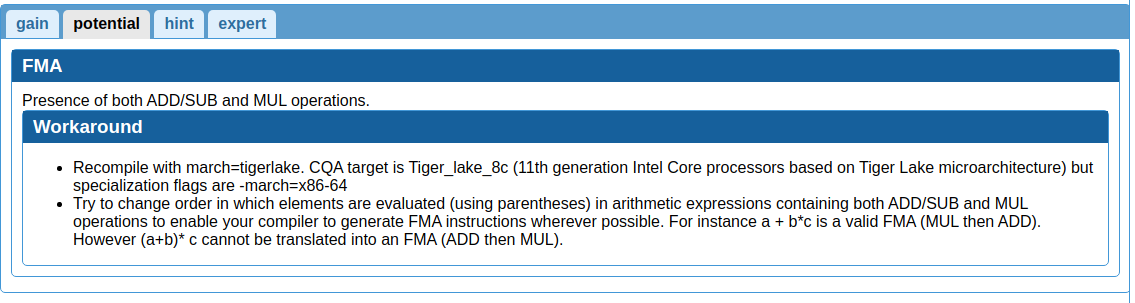
\includegraphics[width=\textwidth]{Figures/cap7.png}
    \caption{Potential : FMA.}
    
    \end{figure}
     \newpage
     \item[\textbullet]\textbf{Hint : Unroll opportunity}
    
    Dans cette section, on nous montre qu'on doit rajouter des options \textbf{ -funroll-loops} et/ou \textbf{-floop-unroll-and-jam} afin d'avoir un meilleur déroulage de boucle.
    
    
    
    
     \begin{figure}[h]
    \centering
    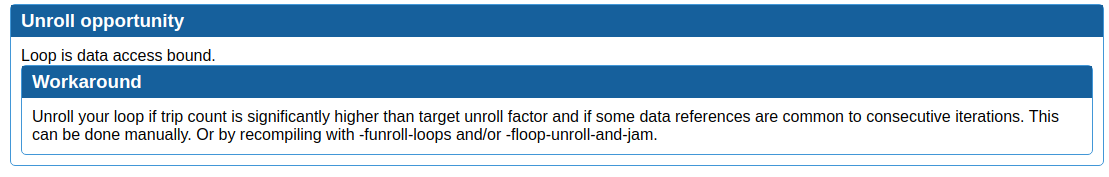
\includegraphics[width=\textwidth]{Figures/cap8.png}
    \caption{Hint : Unroll opportunity.}
    
    \end{figure}
\end{enumerate}
\subsubsection*{La page Summary}   
 Dans cette section, on nous montre qu'on doit rajouter des options d'optimisation et ce qu'on doit changer pour avoir un programme plus performant.
\begin{figure}[h]
    \centering
    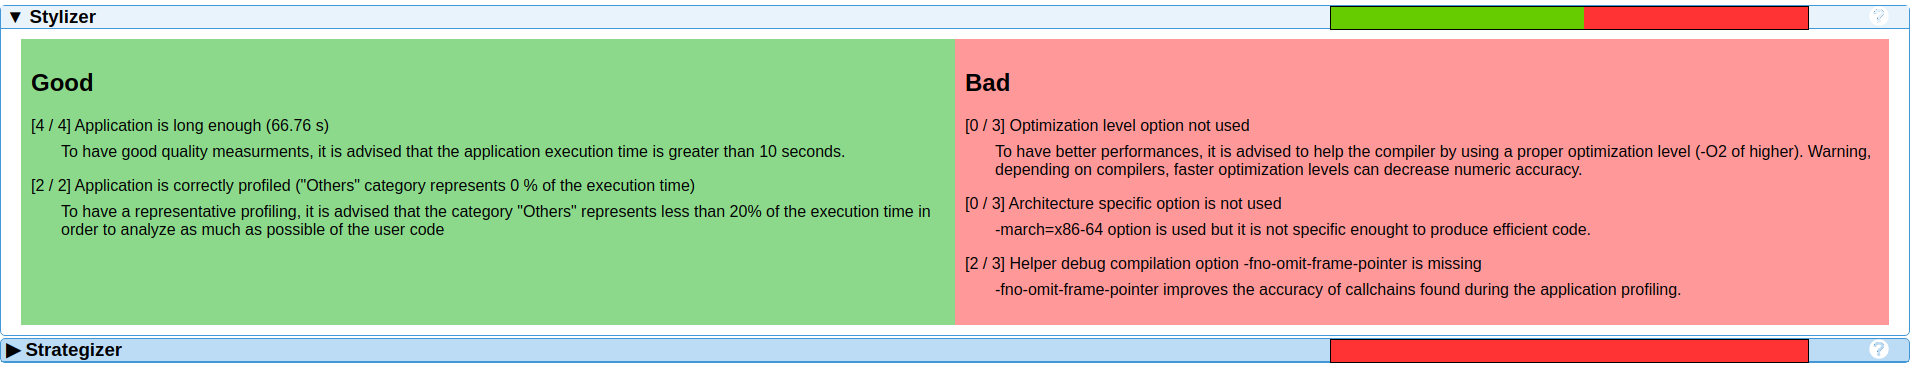
\includegraphics[width=\textwidth,height=7cm]{Figures/cap9.png}
    \caption{Summary :Stylizer.}
    
    \end{figure}
    \newpage
   \subsubsection{Version 1 corrigé de Nbody3D}
   \subsubsection*{Makefile corrigé}
 \begin{customFrame}
all: nbody.g nbody.g1

nbody.g: nbody.c
	gcc -g -mavx2 -fopt-info-all=nbody.gcc.optrpt $< -o $@ -lm -fopenmp

nbody.g1: nbody1.c
	gcc  -mavx2 -funroll-loops -march=tigerlake -finline-functions -fassociative-math -ftree-vectorize -Ofast -g -fopt-info-all=nbody.gcc.optrpt $< -o $@ -lm -fopenmp


clean:
	rm -Rf *~ nbody.g nbody.g1 *.optrpt



\end{customFrame}

 
 \subsubsection*{Code source corrigé}
 Arrivé a cette étape, les principaux changement de notre code source sont les suivants : changement de AOS en SOA et enroulement d'une boucle comme le
montre le code source suivant :

\textbf{Changement en l'ordre de SOA de la fonction init }

\begin{customFrame}

void init(particle_t *p, u64 n)
{
    p->x = malloc(sizeof(f32) * n);
    p->y = malloc(sizeof(f32) * n);
    p->z = malloc(sizeof(f32) * n);
    p->vx = malloc(sizeof(f32) * n);
    p->vy = malloc(sizeof(f32) * n);
    p->vz = malloc(sizeof(f32) * n);
  for (u64 i = 0; i < n; i++)
    {
      //
      u64 r1 = (u64)rand();
      u64 r2 = (u64)rand();
      f32 sign = (r1 > r2) ? 1 : -1;
      
      //
      p->x[i] = sign * (f32)rand() / (f32)RAND_MAX;
      p->y[i] = (f32)rand() / (f32)RAND_MAX;
      p->z[i] = sign * (f32)rand() / (f32)RAND_MAX;

      //
      p->vx[i] = (f32)rand() / (f32)RAND_MAX;
      p->vy[i] = sign * (f32)rand() / (f32)RAND_MAX;
      p->vz[i]= (f32)rand() / (f32)RAND_MAX;
    }
}
\end{customFrame}
\newpage
\textbf{Changement en l'ordre de SOA de la fonction move\_particles }
\begin{customFrame}
void move_particles(particle_t *p, const f32 dt, u64 n)
{
  //
  const f32 softening = 1e-20;

  //
  for (u64 i = 0; i < n; i++)
    {
      //
      f32 fx = 0.0;
      f32 fy = 0.0;
      f32 fz = 0.0;

      //23 floating-point operations
      for (u64 j = 0; j < n; j++)
  {
    //Newton's law
    const f32 dx = p->x[j] - p->x[i]; //1
    const f32 dy = p->y[j] - p->y[i]; //2
    const f32 dz = p->z[j] - p->z[i]; //3
    const f32 d_2 = (dx * dx) + (dy * dy) + (dz * dz) + softening; //9
    const f32 d_3_over_2 = pow(d_2, 3.0 / 2.0); //11

    //Net force
    fx += dx / d_3_over_2; //13
    fy += dy / d_3_over_2; //15
    fz += dz / d_3_over_2; //17
  }

      //
      p->vx[i] += dt * fx; //19
      p->vy[i] += dt * fy; //21
      p->vz[i] += dt * fz; //23
    }

  //3 floating-point operations
  for (u64 i = 0; i < n; i+=4)
    {
      p->x[i] += dt * p->vx[i];
      p->y[i] += dt * p->vy[i];
      p->z[i] += dt * p->vz[i];

      p->x[i+1] += dt * p->vx[i+1];
      p->y[i+1] += dt * p->vy[i+1];
      p->z[i+1] += dt * p->vz[i+1];


      p->x[i+2] += dt * p->vx[i+2];
      p->y[i+2] += dt * p->vy[i+2];
      p->z[i+2] += dt * p->vz[i+2];


      p->x[i+3] += dt * p->vx[i+3];
      p->y[i+3] += dt * p->vy[i+3];
      p->z[i+3] += dt * p->vz[i+3];
    }
}
\end{customFrame}
\textbf{Changement de l'enroulement de la boucle}
\begin{customFrame}
for (u64 i = 0; i < n; i+=4)
    {
      p->x[i] += dt * p->vx[i];
      p->y[i] += dt * p->vy[i];
      p->z[i] += dt * p->vz[i];

      p->x[i+1] += dt * p->vx[i+1];
      p->y[i+1] += dt * p->vy[i+1];
      p->z[i+1] += dt * p->vz[i+1];


      p->x[i+2] += dt * p->vx[i+2];
      p->y[i+2] += dt * p->vy[i+2];
      p->z[i+2] += dt * p->vz[i+2];


      p->x[i+3] += dt * p->vx[i+3];
      p->y[i+3] += dt * p->vy[i+3];
      p->z[i+3] += dt * p->vz[i+3];
    }
\end{customFrame}
\textbf{Libérer les allocations}
\begin{customFrame}
    free(p->x);
    free(p->y);
    free(p->z);
    free(p->vx);
    free(p->vy);
    free(p->vz);
\end{customFrame}
\newpage

\subsubsection*{Résultats obtenues}
Après éxecution du programme, on remarque notre programme est améliorer avec des speedup de 1.0 , une vectorisation à 100\%, les options de compilation qui sont complètes, comme on le voit dans les figures suivantes:

\begin{enumerate}
    \item[1.]\textbf{La page index : }
   On voit clairement que notre programme est totalement vectorisé et est au plus efficace possible : gain de temps d'exécution constaté
    par rapport à toutes la version de base précédente. Nous avons donc ainsi atteint le meilleur code possible avec les meilleurs options d'optimisation possible pour le Nbody3D. 
    \begin{figure}[h]
    \centering
    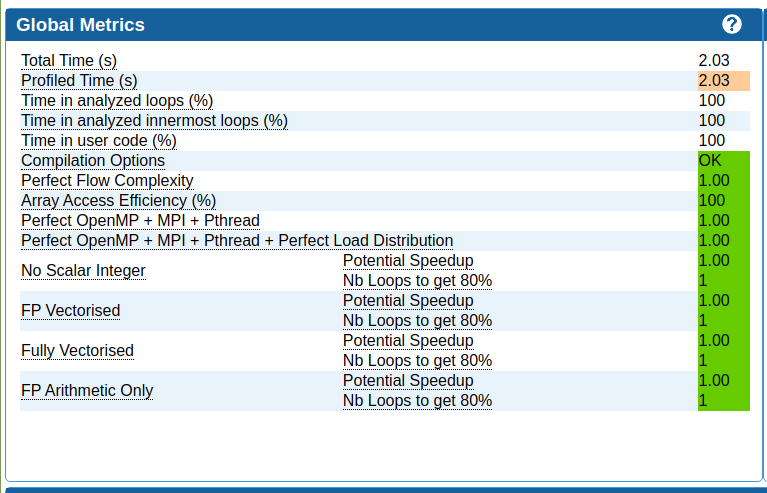
\includegraphics[width=\textwidth]{Figures/cap10.png}
    \caption{Global Metrics de la version optimisé.}
    
    \end{figure}
   \item[2.]\textbf{La page Loops}
   
   On voit que les parameètres sont très suffisant, il manque la Vectorization Efficiency, on consulte son rapport CQA afin de voir les modifications qu'il faut apporter.
   \begin{figure}[h]
    \centering
    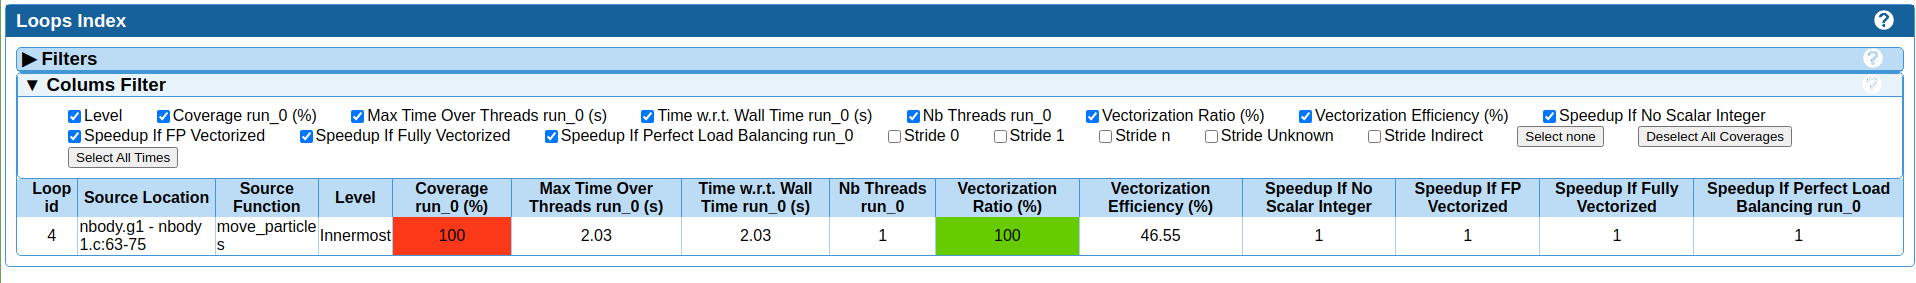
\includegraphics[width=\textwidth]{Figures/cap11.png}
    \caption{Loops Index de la version 1 optimisé.}
    
    \end{figure}
  \newpage
     \item[3.]\textbf{La page Summary}
     
     \begin{figure}[h]
    \centering
    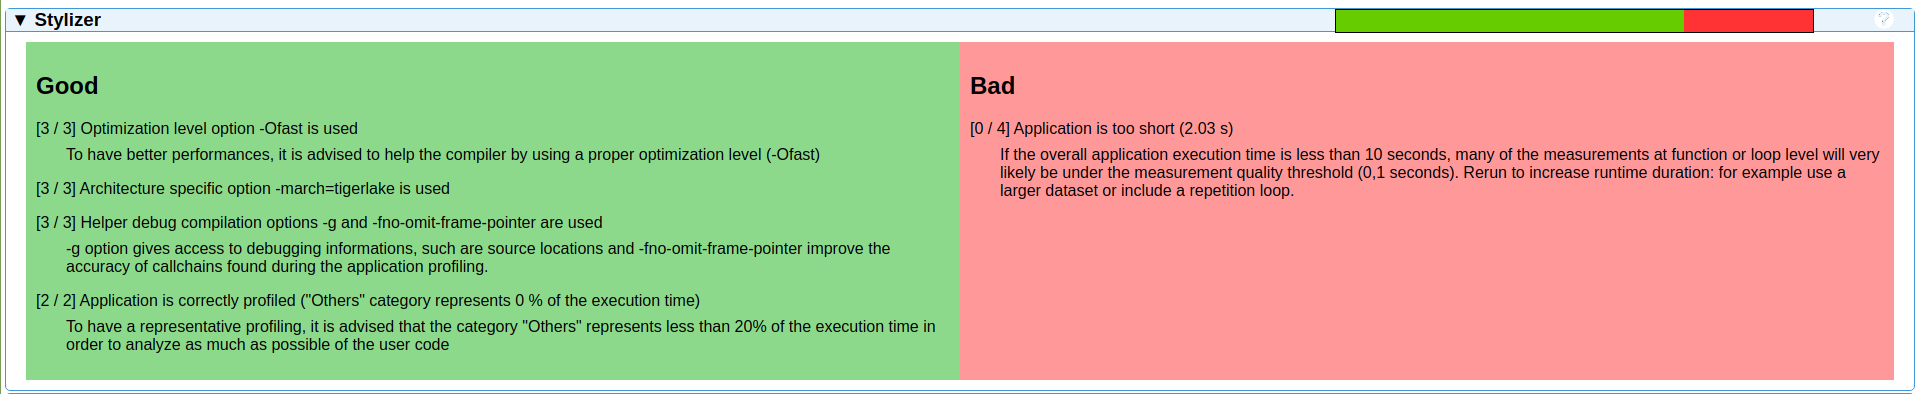
\includegraphics[width=\textwidth]{Figures/cap12.png}
    \caption{Summary : Stylizer de la version 1 optimisé.}
    
    \end{figure}
    
    \item[3.]\textbf{Rapport CQA}
     \begin{enumerate}
         \item[\textbullet] \textbf{Gain : }
         On voit que notre boucle est vectorisé, mais que 46\% de la longueur du registre.
         \begin{figure}[h]
    \centering
    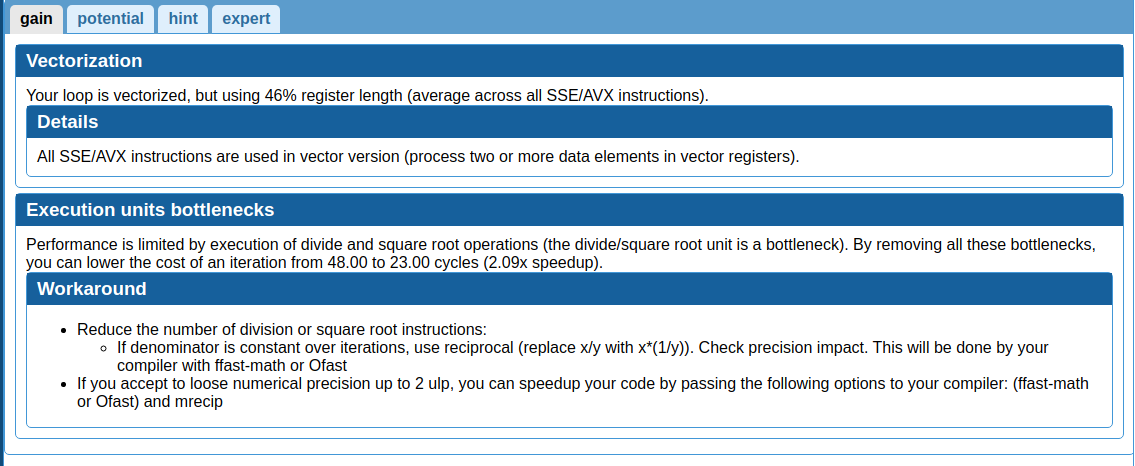
\includegraphics[width=\textwidth]{Figures/cap13.png}
    \caption{Gain de la version 1 optimisé.}
    
    \end{figure}
    \newpage
         \item[\textbullet] \textbf{Hint : Vector unaligned load/store instructions}
         
         D'après les sections du rapport suivante, on se rend compte que notre programme est vectorisé mais pas totalement. Ce problème vient du fait que notre mémoire n'est pas alignée et nous applicons donc la suggestion d'utiliser la fonction \textbf{posix\_memalign} . 
         \begin{figure}[h]
    \centering
    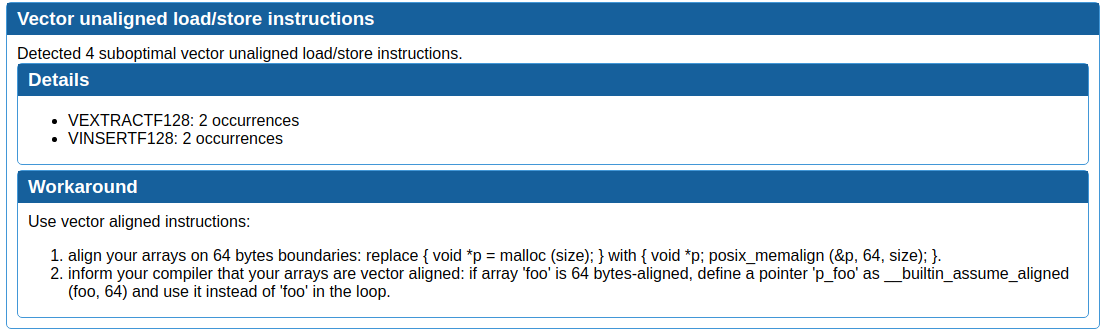
\includegraphics[width=\textwidth]{Figures/cap15.png}
    \caption{Vector unaligned load/store instructions de la version 1 optimisé.}
    
    \end{figure}
        
     \end{enumerate}
    
\end{enumerate}
\end{document}